\documentclass{jsarticle}
\usepackage[dvipdfmx]{graphicx}

\title{フロンティア法プログラム}

\begin{document}

\maketitle

\section{はじめに}

フロンティア法は、与えられたグラフ上において、指定された2点間のパスや全域木、
連結成分などを表現するZDDを構築するアルゴリズムである。
構築したZDDを基に、全解の列挙や数え上げ、ランダムサンプリングなどを行える。

以下では、パスや全域木など、ZDDで表現したい部分グラフを構築対象と呼ぶ。

\section{できること}

\begin{itemize}
\item 入力グラフに対して、以下の部分グラフ(構築対象)の全てを表現するZDDの構築
\begin{itemize}
\item 全域森
\item 全域木
\item 無向 $s$-$t$ パス(サイクル)
\item 有向 $s$-$t$ パス(サイクル)
\item (無向)辺素 $s$-$t$ パス(サイクル)
\item 根付き森
\item 連結成分
\item $k$-カット (高々 $k$ 本のカット)
\item 源を指定したカット
\end{itemize}
\item 入力ハイパーグラフに対して、以下の部分ハイパーグラフ(構築対象)の全てを表現するZDDの構築
\begin{itemize}
\item 集合分割
\item 集合被覆
\item 集合パッキング
\end{itemize}
\item 構築したZDDの既約化(reduced and ordered ZDD を得る)
\item 構築したZDDの解の個数のカウント
\item 構築したZDDから全解を列挙
\item 構築したZDDから解の一様ランダムサンプリング
%\item 構築したZDDのオートマトン化
\item 入力グラフの頂点番号を幅優先順に付け替え
\item 入力グラフ、出力ZDDのgraphviz形式~\footnote{グラフ描画プログラム。http://graphviz.org/}による出力
\end{itemize}

\section{ビルドと実行}

\subsection{準備}

64ビット整数(32ビット整数)で表現できない大きな数を扱うときは、
GNU MPライブラリ(\texttt{http://gmplib.org/})をあらかじめインストールしておくと良い。
ただし、インストールしなくても差し支えは無い(\ref{sec:precision}~節参照)。

\subsection{ビルド}

\texttt{./configure} と \texttt{make} によって導入する。

\begin{verbatim}
./configure
make
\end{verbatim}

オプションを指定しない場合、64ビット版がビルドされる。
32ビット版をビルドする場合は以下で示すようにオプションを与える。

\begin{verbatim}
./configure --enable-32bit
make
\end{verbatim}

\texttt{src/frontier} ディレクトリに \texttt{frontier}、 \texttt{enumpath} プログラムと
\texttt{libfrontier.a} ライブラリファイルが生成される。
また、\texttt{utility} ディレクトリに \texttt{makegrid} プログラムが生成される。
\texttt{make install} コマンドでこれらのプログラムをインストールすることができる。

説明の都合上、プログラムを展開したディレクトリの直下にシンボリックリンクを張る。

\begin{verbatim}
ln -s src/frontier/frontier frontier
ln -s src/utility/makegrid makegrid
\end{verbatim}

\texttt{makegrid} プログラムは $m \times n$ グリッドグラフを生成する。
\texttt{frontier} プログラムの入力として用いることができる。

実行例($2 \times 3$ グリッドグラフの生成)

\begin{verbatim}
./makegrid 2 3
\end{verbatim}

出力

\begin{verbatim}
2 4
1 3 5
2 6
1 5
2 4 6
3 5
\end{verbatim}

\subsection{実行例}

$3 \times 3$ グリッドの全域森ZDDを構築するには、以下のコマンドを実行する。

\begin{verbatim}
./makegrid 3 3 | ./frontier -t sforest
\end{verbatim}

標準出力の結果

\begin{verbatim}
#1:
2:3,4
#2:
3:5,5
4:5,6
#3:
5:7,8
...
\end{verbatim}

上記の出力はZDDを表す。出力の見方は \ref{sec:outputzdd} 節を参照。

標準エラー出力の結果

\begin{verbatim}
# of nodes of ZDD = 45
# of solutions = 3102
\end{verbatim}

構築したZDDの既約化前のノード数は45、解の数(ZDDが表現する集合族の要素の個数)は
3,102であることがわかる。

ZDDを既約化するには \texttt{-r} オプションを用いる。

\begin{verbatim}
./makegrid -d 3 3 | ./frontier -t sforest -r
\end{verbatim}

出力結果(ZDD本体は省略)

\begin{verbatim}
# of nodes of ZDD = 45
# of nodes of reduced ZDD = 38
# of solutions = 3102
\end{verbatim}

$s$-$t$パスZDDを構築するには \texttt{-t stpath} オプションを用いる。
以下のコマンド例は、$3 \times 3$ グリッドの1つの角から対角の角までの
全パスのZDDを構築する。始点を指定しない場合は頂点番号1、
終点を指定しない場合は最も大きな頂点番号を指定したことになる。
$3 \times 3$ グリッドの場合は始点は頂点1、終点は頂点9となる。
%\texttt{makegrid} ユーティリティのドキュメントも参照のこと。

\begin{verbatim}
./makegrid -d 3 3 | ./frontier -t stpath
\end{verbatim}

$s$-$t$パスの始点番号は \texttt{-s} オプションで、
終点番号は \texttt{-e} オプションで指定する。

\begin{verbatim}
./makegrid -d 3 3 | ./frontier -t stpath -s 2 -e 8
\end{verbatim}


\section{入力書式}

\texttt{frontier} プログラムに与える入力は、無向グラフ、有向グラフ、ハイパーグラフのいずれかであり、
\texttt{-t} オプションで指定した構築対象によって異なる。
いずれの形式でも、頂点番号、辺の番号はともに1から始まる。

\subsection{無向グラフの入力書式}

無向グラフを入力する場合、隣接リスト形式または辺リスト形式のテキストで表されたグラフを入力する。
隣接リスト形式を指定する場合はオプション無しであり、
辺リスト形式を用いる場合は \texttt{-c} オプションを指定する。

隣接リスト形式では$i$行目に頂点$i$に隣接する頂点の番号を並べる。
隣接リスト形式では、並列辺(parallel edge)は無視される。
すなわち、頂点 $i$ から $j$ に張られた辺が複数存在する入力を与えた場合も、
1本しか存在しないグラフに変換される。
したがって、$i$ 行目に$j$が記述され、$j$行目に$i$が記述されているとき、
入力を読み込んで作成されるグラフでは、
$i$, $j$ 間には辺が1本だけ存在する($j$行目の$i$の記述は無視されると考える)。
辺の番号は、無視される辺を除いて、
隣接リストでの番号の出現順に$1,2,3,\ldots$ と振られる
(フロンティア法ではこの順で辺が処理される)。
隣接リスト形式では、辺の番号(順番)を自由に指定することはできない。
辺の番号を指定する場合は辺リスト形式を用いる必要がある。

辺リスト形式では、1行目に頂点の個数を書き、2行目以降の各行に辺の始点と終点番号を並べる。
辺リスト形式では、並列辺は無視されない。

図~\ref{fig:graph_example}のグラフを例に考える。

\begin{figure}[h]
  \begin{center}
    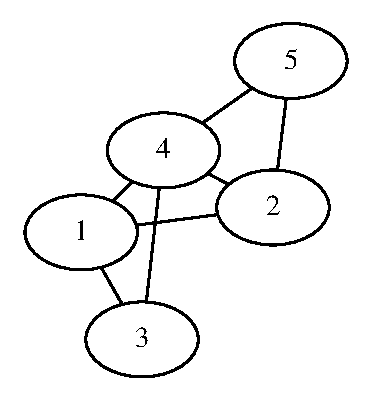
\includegraphics[width=40mm]{graph_example.eps}
  \end{center}
  \caption{入力グラフの例}
  \label{fig:graph_example}
\end{figure}

図~\ref{fig:graph_example}のグラフを表現する隣接リストは以下の通りである。

\begin{verbatim}
2 3 4
4 5
4
5

\end{verbatim}

このとき、$i$ 番の辺$e_i$ は、$e_1 = \{1, 2\}$, $e_2 = \{1, 3\}$, $e_3 = \{1, 4\}$,
$e_4 = \{2, 4\}$, $e_5 = \{2, 5\}$, $e_6 = \{3, 4\}$, $e_7 = \{4, 5\}$ となる。

図~\ref{fig:graph_example}のグラフを表現する辺リストは以下の通りである。

\begin{verbatim}
5
1 2
1 3
1 4
2 4
2 5
3 4
4 5
\end{verbatim}

辺に重みを付けることも可能である。3番目の数字が辺の重みとなる。
3番目の数字が省略された場合、重みは1とみなされる。

\begin{verbatim}
5
1 2 3.2
1 3 4.5
1 4 1.7
2 4 9.6
2 5 12.0
3 4 23.1
4 5 32.0
\end{verbatim}

辺に重みを付ける場合、隣接リストは用いることができない。

\subsection{有向グラフの入力書式}

入力が有向グラフの場合、... (未稿)

\subsection{ハイパーグラフの入力書式}

入力がハイパーグラフの場合、... (未稿)

\subsection{入力グラフの確認}

用意した入力が意図した通りに \texttt{frontier} プログラムに読み込まれるかを確認するために、
\texttt{--print-graph-al}, \texttt{--print-graph-el},
\texttt{--print-graphviz} オプションが用意されている。\texttt{--print-graph-al} は
入力グラフを隣接リスト形式で、\texttt{--print-graph-el} は入力グラフを
辺リスト形式で出力する。このオプションを用いることで、
隣接リスト形式と辺リスト形式の相互変換も可能である。
\ref{sec:option} 節のオプションリストも参照のこと。

例:入力グラフを辺リスト形式で標準出力に出力する。
\begin{verbatim}
./makegrid 3 | ./frontier --print-graph-el -
\end{verbatim}

例:入力グラフを隣接リスト形式でファイル xxx.txt に出力する。
\begin{verbatim}
./makegrid 3 | ./frontier --print-graph-al xxx.txt
\end{verbatim}

\texttt{--print-graphviz} オプションは入力グラフを
graphviz 形式で出力する。graphviz をインストールしていれば、
グラフを描画することができる。辺の番号を確認するときなどに使うことができる。

例:入力グラフをgraphvizで描画(pngフォーマットで出力)
\begin{verbatim}
./makegrid 3 | ./frontier --print-graphviz - | neato -Tpng -o xxx.png
\end{verbatim}

出力結果は図~\ref{fig:graphviz_example} のようになる。

\begin{figure}[h]
  \begin{center}
    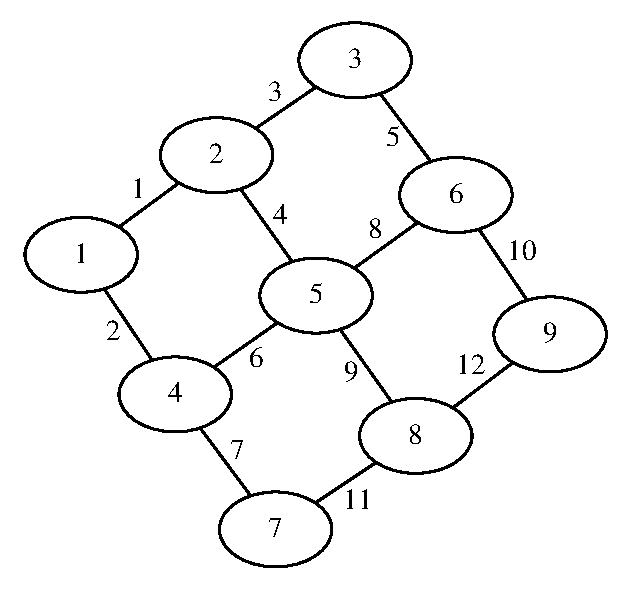
\includegraphics[width=40mm]{graphviz_example.eps}
  \end{center}
  \caption{graphviz形式による出力例}
  \label{fig:graphviz_example}
\end{figure}

\section{出力書式}

\subsection{ZDDの出力} \label{sec:outputzdd}

\texttt{frontier} プログラムは、標準出力にZDDを出力する。

出力ZDDの例

\begin{verbatim}
#1:
2:3,4
#2:
3:5,5
4:5,6
#3:
5:7,8
...
\end{verbatim}

\texttt{\#i:} の行は、変数(辺)番号\texttt{i}の変数が始まることを意味する。
\texttt{p:q,r} の行は、ノード番号 \texttt{p} の0-枝の先がノード番号 \texttt{q} に、
1-枝の先がノード番号 \texttt{r} に接続していることを意味する。
0-終端は番号0、1-終端は番号1であり、終端以外のノードは2以上の番号をもつ。
ノード番号はデフォルトでは10進数であるが、\texttt{--hex} オプションを与えると
16進数(Knuthの形式)にすることができる。

プログラムに \texttt{-r} オプションを与えると既約なZDDが出力される。

\subsection{graphvizによるZDDの描画}

graphviz プログラムを用いてZDDを描画することができる。
\texttt{--print-zdd-graphviz} オプションでgraphviz形式のZDDを出力できる。

例:$s$-$t$パスを表すZDDをgraphvizで描画(pngフォーマットで出力)

\begin{verbatim}
./makegrid 3 | ./frontier -t stpath -n --print-zdd-graphviz - | dot -Tpng -o xxx.png
\end{verbatim}

出力結果は図~\ref{fig:zdd_example} のようになる。

\begin{figure}[h]
  \begin{center}
    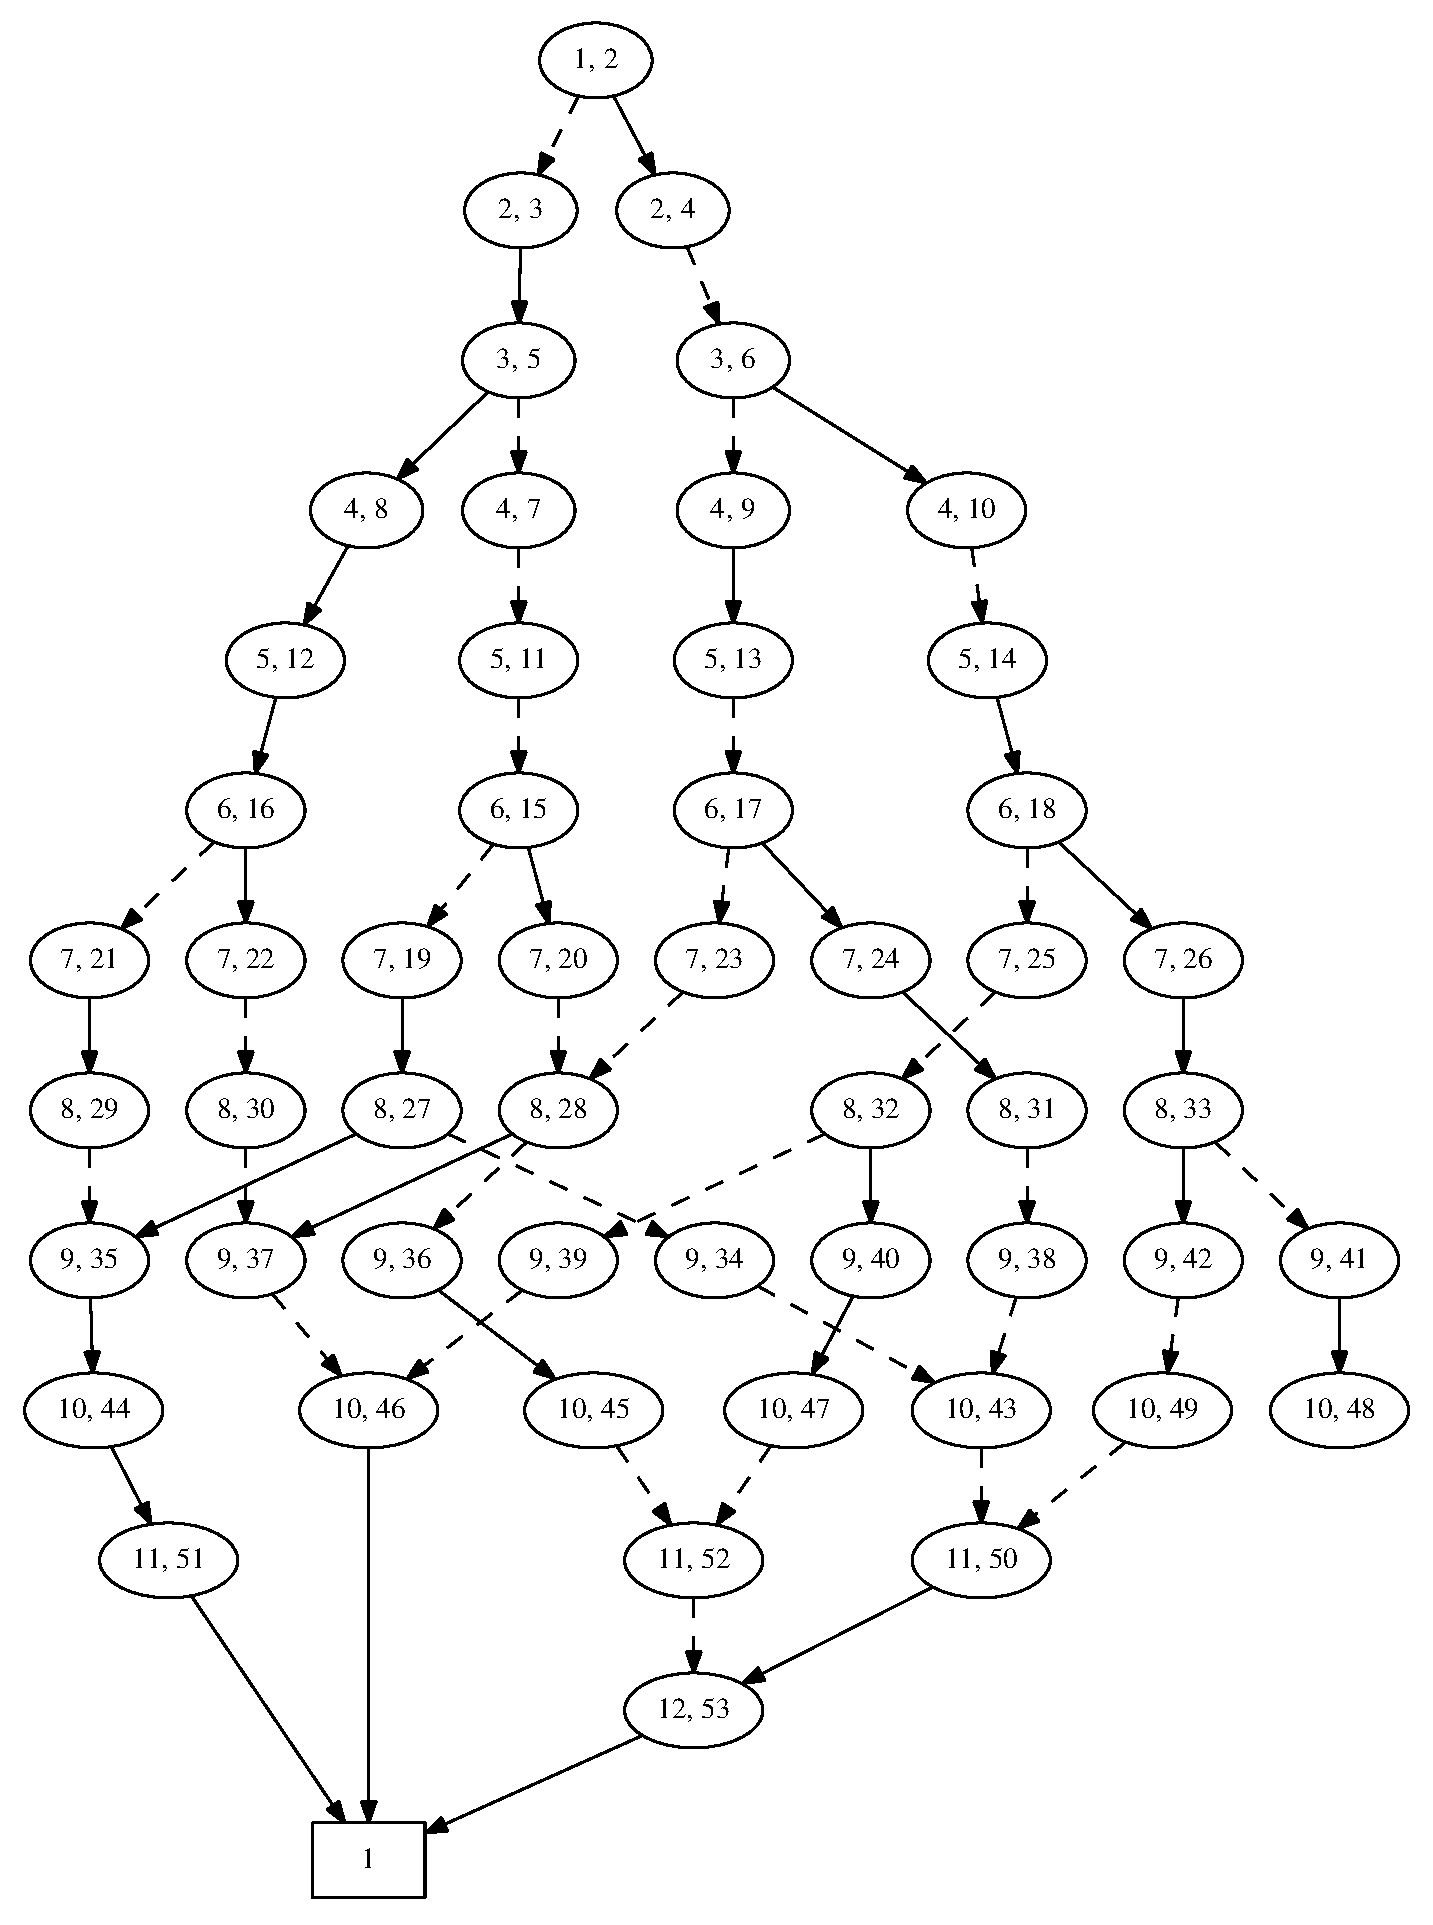
\includegraphics[width=40mm]{zdd_example.eps}
  \end{center}
  \caption{graphviz形式によるZDDの描画例}
  \label{fig:zdd_example}
\end{figure}

\subsection{要素の列挙、一様ランダムサンプリング}

\texttt{--enum} オプションでZDDが表現する集合族の全集合の列挙、\texttt{--sample} オプションで
全集合から一様にランダムサンプリングができる。

例:$s$-$t$パス(の辺集合)を全列挙

\begin{verbatim}
./makegrid 3 | ./frontier -t stpath -n --enum -
\end{verbatim}

出力例

\begin{verbatim}
1 3 5 6 7 8 11 12
1 3 5 8 9 12
1 3 5 10
1 4 6 7 11 12
1 4 8 10
1 4 9 12
2 3 4 5 6 10
2 3 4 5 7 9 10 11
2 6 8 10
2 6 9 12
2 7 8 9 10 11
2 7 11 12
\end{verbatim}

1行が1つの集合に対応する。上記の出力は $\{1,3,5,6,7,8,11,12\},\{1,3,5,8,9,12\},\ldots$ を表す。

例:$s$-$t$パスの一様ランダムサンプリング(20個)

\begin{verbatim}
./makegrid 3 | ./frontier -t stpath -n --sample - 20
\end{verbatim}

\subsection{計算精度}\label{sec:precision}

ZDDの解の個数が64ビットまたは32ビットで表現できる数($2^{64} - 1$または$2^{32} - 1$)
を超える数を扱うには、GNU MPライブラリ、または、
同梱のBigIntegerを用いる。

本プログラムのビルド時(./configure 実行時)
GMPライブラリがインストールされていると、
自動的にリンクされ、使用可能となる。
特別な設定を何もしなくても(オプションを何もつけなくても)
GMPライブラリが使用される。

GMPライブラリがインストールされていない場合、
BigIntegerが使用される。

以下で説明するオプションは、特殊な事情が無い限り付加する必要は無いと思われる。
\texttt{--sm}オプションを用いるとGMPライブラリが、
\texttt{--sb}オプションを用いるとBigIntegerが強制使用される。
\texttt{--sd}オプションを用いると、double型による計算を行う。
\texttt{--si}オプションを用いると、64ビットまたは32ビット整数型による計算を行う。
\texttt{--si}オプションは、メモリの使用量は最も少ないが、
計算結果のオーバーフローが起こる可能性があり、大きな数を正しく扱えないことに注意。

旧バージョンで使用していたapfloatライブラリは廃止された。代わりにGMPライブラリを用いる。

\section{オプション}\label{sec:option}

\subsection{構築対象}

構築対象は \texttt{-t} \textit{kind} の形式で指定する。
\textit{kind} に指定可能な対象を表~\ref{tab:kind}に示す。

\begin{table}
\caption{構築対象の指定}
\label{tab:kind}
\begin{center}
\begin{tabular}[t]{|l|l|l|}
\hline
\textit{kind} & 入力 & 構築対象 \\ \hline \hline
\texttt{sforest} & 無向グラフ &全域森 (spanning forest) \\ \hline
\texttt{stree} & 無向グラフ & 全域木 (spanning tree) \\ \hline
\texttt{stpath} & 無向グラフ & 無向 $s$-$t$ パス ($s$-$t$ path) \\ \hline
\texttt{pathmatching} or \texttt{pm} & 無向グラフ & パスマッチング(複数パス) \\ \hline
\texttt{mtpath} or \texttt{numberlink} & 無向グラフ & 複数終端対パス (multi terminal paths) \\ \hline
\texttt{dstpath} & 有向グラフ & 有向 $s$-$t$ パス (directed $s$-$t$ path) 現バージョンでは未対応 \\ \hline
\texttt{stedpath} & 無向グラフ & (無向)辺素 $s$-$t$ パス (edge-disjoint $s$-$t$ path) 現バージョンでは未対応 \\ \hline
\texttt{rforest} & 無向グラフ & 根付き森 (rooted forest) \\ \hline
\texttt{comp} & 無向グラフ & 連結成分 (component) \\ \hline
\texttt{kcut} & 無向グラフ & $k$-カット ($k$-cut) \\ \hline
\texttt{rcut} & 無向グラフ & 源を指定した $k$-カット (terminal $k$-cut) \\ \hline
\texttt{setpt} & ハイパーグラフ & 集合分割 (set partition) \\ \hline
\texttt{setc} & ハイパーグラフ & 集合被覆 (set cover) \\ \hline
\texttt{setpk} & ハイパーグラフ & 集合パッキング (set packing) \\
\hline
\end{tabular}
\end{center}
\end{table}

\subsection{オプション}

プログラムのオプションを表~\ref{tab:option}, \ref{tab:option2}に示す。表の
「使用可能構築対象」は、そのオプションが使用可能な構築対象である。
例えば、\texttt{--cycle} オプションは無向パス、有向パス列挙時(\textit{kind} が
\texttt{stpath} または \texttt{dstpath})にのみ使用可能である。
一部のオプションでは引数に \textit{filename} (ファイル名)を指定することが
あるが、\texttt{-} を指定することで標準出力に出力することができる。

\begin{table}
\caption{プログラムのオプション}
\label{tab:option}
\begin{center}
\begin{tabular}[t]{|p{120pt}|p{50pt}|p{80pt}|p{180pt}|}
\hline%
オプション & デフォルト & 使用可能構築対象 & 効果 \\ \hline \hline
\texttt{-t} \textit{kind} & \texttt{sforest} & 全て & 列挙の種類を指定する。
                            \textit{kind} に指定する内容は表~\ref{tab:kind}を参照。 \\ \hline
\texttt{-b} & off & 入力がグラフである構築対象全て & 入力されたグラフについて、
                    始点からの幅優先探索によって頂点番号を付け替える。 \\ \hline
\texttt{--input-al} & on & 入力がグラフである構築対象全て & 入力として、隣接リスト形式を用いる。 \\ \hline
\texttt{-c} or \texttt{--input-el} & off & 入力がグラフである構築対象全て & 入力として、辺リスト形式を用いる。 \\ \hline
\texttt{-w} or \texttt{--weight} \textit{filename} & 指定しない & 全て & 辺に重みを設定する。ファイル \textit{filename} には数字(double型)の列を記入する。前から順に辺に重みが設定される。書かれた数字が辺の個数より少ない場合、残りの辺には1の重みが設定される。入力グラフに記述された重みより、本オプションで指定した重みが優先される。 \\ \hline
\texttt{-s} $N$ & 1 & \texttt{stpath}, \texttt{dstpath} & 始点の頂点番号を $N$ に設定する。 \\ \hline
\texttt{-e} $N$ & 最大頂点番号 & \texttt{stpath}, \texttt{dstpath} & 終点の頂点番号を $N$ に設定する。 \\ \hline
\texttt{-h} or \texttt{--hamilton}& off & \texttt{stpath}, \texttt{dstpath} & $s$-$t$ パス、サイクル列挙時にハミルトンパス、サイクルを列挙する。 \\ \hline
\texttt{--cycle} & off & \texttt{stpath}, \texttt{dstpath} & サイクルを列挙する。 \\ \hline
\texttt{--any} & off & \texttt{stpath}, \texttt{dstpath} & 始点から任意の頂点へのパスを列挙する。 \\ \hline
\texttt{-k} or \texttt{--upper} $D$ & $\infty$ & \texttt{comp}, \texttt{kcut}, \texttt{rcut}, \texttt{stpath} & カット列挙において、カットの数を指定。連結成分列挙において、連結成分の数を指定。また、パス列挙において、パスの長さの上限を指定。\texttt{--le} オプションを指定すると重さの総和が高々 $D$ の対象を列挙。\texttt{--me} オプションを指定すると重さの総和が少なくとも $D$ の対象を列挙。\texttt{--le}  \texttt{--me} のいずれも指定しない場合は重さの総和がちょうど $D$ の対象を列挙。 \\ \hline
\texttt{--le} & off & \texttt{comp}, \texttt{kcut}, \texttt{rcut}, \texttt{stpath} & \texttt{-k} オプションと同時に指定することで、重さの総和が高々 $D$ の対象を列挙。 \\ \hline
\texttt{--me} & off & \texttt{comp}, \texttt{kcut}, \texttt{rcut}, \texttt{stpath} & \texttt{-k} オプションと同時に指定することで、重さの総和が少なくとも $D$ の対象を列挙。 \\ \hline
\end{tabular}
\end{center}
\end{table}

\begin{table}
\caption{プログラムのオプション(続き)}
\label{tab:option2}
\begin{center}
\begin{tabular}[t]{|p{120pt}|p{50pt}|p{80pt}|p{180pt}|}
\hline%
オプション & デフォルト & 使用可能構築対象 & 効果 \\ \hline \hline
\texttt{-f} $r_1$ $r_2$ $\cdots$ & 指定なし & \texttt{rforest}, \texttt{rcut} & 根付き木、源を指定したカットの列挙において、根や源の頂点番号 $r_1, r_2,\ldots$ を指定。\\ \hline
\texttt{--root} \textit{filename} & 指定なし & \texttt{rforest}, \texttt{rcut} & 根付き木、源を指定したカットの列挙において、根や源の頂点番号を指定。\texttt{-f} オプションとは異なり、ファイルから読み込む。ファイル \textit{filename} には数字(double型)の列を記入する。 \\ \hline
\texttt{-r} & off & 全て & 構築したZDDを既約化する。\\ \hline
\texttt{-n} or \texttt{--no-print-zdd} & off(出力する) & 全て & ZDDを標準出力に出力しないようにする。\texttt{>/dev/null} と同様だが、本オプションの方が高速。 \\ \hline
\texttt{--terminal} \textit{filename} & off & \texttt{mtpath} & 複数終端対パスの列挙において、終端対を記述したファイルを指定する。ファイル \textit{filename} には数字(int型)の列を、始点と終点を交互に記入する。 \\ \hline
\texttt{--print-zdd-graphviz} \quad \textit{filename} [\texttt{0}] & off(出力しない) & 全て & ZDDをgraphviz形式でファイル(標準出力)に出力する。第2引数に\texttt{0}を指定すると0-終端も印字する(指定しない場合は0-終端は印字されない)。 \\ \hline
\texttt{--print-zdd-sbdd} \quad \textit{filename} [\texttt{0}] & off(出力しない) & 全て & ZDDをSapporoBDD library の Import 関数で読み込める形式でファイル(標準出力)に出力する。 \\ \hline
\texttt{--no-solution} & off(計算する) & 全て & ZDDの解の個数を計算しない。 \\ \hline
\texttt{--print-graph-al} \textit{filename} & off & 全て & 入力グラフを隣接リスト形式でファイル(標準出力)に出力して、プログラムを終了する。デバッグ用。 \\ \hline
\texttt{--print-graph-el} \textit{filename} & off & 全て & 入力グラフを辺リスト形式でファイル(標準出力)に出力して、プログラムを終了する。デバッグ用。 \\ \hline
\texttt{--print-graphviz} \textit{filename} & off & 全て & 入力グラフをgraphviz形式でファイル(標準出力)に出力して、プログラムを終了する。 \\ \hline
\end{tabular}
\end{center}
\end{table}

\begin{table}
\caption{プログラムのオプション(続き)}
\label{tab:option3}
\begin{center}
\begin{tabular}[t]{|p{120pt}|p{50pt}|p{80pt}|p{180pt}|}
\hline%
オプション & デフォルト & 使用可能構築対象 & 効果 \\ \hline \hline
\texttt{--enum} \textit{filename} & off & 全て & ZDDの全解をファイル(標準出力)に出力する。出力形式は下記参照。 \\ \hline
\texttt{--sample} \textit{filename} [$N$] & off & 全て & ZDDの全解から一様ランダムサンプリングを行い、$N$個の解をファイル(標準出力)に出力する。$N$のデフォルト値は100。出力形式は下記参照。 \\ \hline
\texttt{--hex} & off & 全て & ZDDの出力時、ID番号を16進数にする(Knuth の形式)。 \\ \hline
\texttt{--am} & off & 全て & ZDDをオートマトンに変換する。\\ \hline
\texttt{--print-am} & off & 全て & オートマトンを出力する。 \\ \hline
\texttt{-v} & off & 全て & 計算の途中経過を印字する。\\ \hline
\texttt{--si} & off & 全て & 解の数の計算において、64ビットまたは32ビット型整数を用いる。オーバーフローの検知は行わない。\\ \hline
\texttt{--sd} & off & 全て & 解の数の計算において、double 型を用いる。\\ \hline
\texttt{--sb} & off & 全て & 解の数の計算において、BigInteger型(任意長整数型)を用いる。\\ \hline
\texttt{--sm} & off & 全て & 解の数の計算において、GMPライブラリを用いる。\\ \hline
\texttt{--sa} & off & 全て & 解の数の計算において、apfloatライブラリを用いる(廃止)。\\ \hline
\end{tabular}
\end{center}
\end{table}

\end{document}
